Computer assisted drug design seeks to extend rational drug design by making use of the continuously increasing processing power available both in high performance super computers, but also in single workstations.
Seeking to supplement the ability of a researcher either by allowing examination of a large number of possible interactions quickly or providing some insight that might be much more difficult to obtain through biochemical experiments, both in terms of time and expense.
Different classes of programs seek to help solve each of the distinct steps in the pre-clinical stages of drug development, namely:
\begin{enumerate}
\item Hit Identification – the process of screening a large small molecule database (up to one million or more small molecules) database to identify small molecules which bind a given target protein, or hits.
\item Hit to lead optimization - the process of modifying these ``hit'' molecules either by substitution or addition of chemical moieties or mixing and matching substructures between given hits, to produce compounds with higher binding affinities than the initial hit compounds.
\item Lead Optimization – the final step of modifying lead compounds to increase ``druglikeness'' to ensure that the molecule is sufficiently soluble, well tolerated, and does not disrupt regular cellular function.
\end{enumerate}

Hit identification has evolved from first animal screens, where mutant animals were studied to find the specific gene or protein causing a specific phenotype.
Because of the cost and time required in animal screens, even with exhaustive mutation and deletion libraries for organisms such as yeast and {\it Escherichia coli}, these screens are slow, often taking three years or longer, and error prone, as performing a large number of repetitive experiments causes even the most fastidious of scientists to lose focus.
High-throughput screening seeks to supplement the human factor with robots, which are capable of performing similar experiments with greater speed and fewer errors.
With the help of this automation it is possible to test the interactions of as many as 100 million different reactions per day \cite{agresti2010ultrahigh}.
Though the high initial cost of high-throughput screening equipment as well as the cost of the small molecule libraries necessary for screening are often prohibitive even to large research institutions.
In order to make this sort of experiment available to a larger number of institutions some research institutions have instituted means of sharing this equipment, through high-throughput screening as a service type arrangements \cite{htsrc,mssr}.
The computational equivalent to high-throughput screening is virtual screening.

The problem of the cost of small molecule libraries is essentially a solved problem in virtual screening as there are readily available libraries of drug-like small molecules for use in virtual screening programs.
For example, the ZINC database provides a library of over seven-hundred thousand commercially available small molecules in a number of different file formats for use in virtual screening \cite{irwin2005zinc}.

 \cite{kitchen2004docking}

The first published study using computational docking was published in 1982 by Irwin Kuntz describing a program which would later go on to become the well known DOCK program \cite{kuntz1982geometric}.
Generally docking consists of a method of quickly screening possible protein-small-molecule interaction conformations.
An emphasis is placed on the computational cost of evaluating the energy function over accuracy, as the poses generated by this step are usually fed into structural refinement programs for further sampling and more accurate estimation of energies.
For example in the original Kuntz study, the system only only had six degrees of freedom on which to sample, three translational and three rotational degrees of freedom for the ligand with the protein held fixed.
Along with a hard sphere collision model this provided a sufficiently selective screen to identify the native binding geometry of the heme group to myoglobin as well as thyroid hormone analogs to prealbumin. 
 \cite{kuntz1982geometric}

The rate at which new structures are being deposited into the Protein Data Bank is increasing on an annual basis.
But tools are necessary to draw meaningful insights from this data, hopefully leading to new drugs.

\begin{figure}[H]
\begin{center}
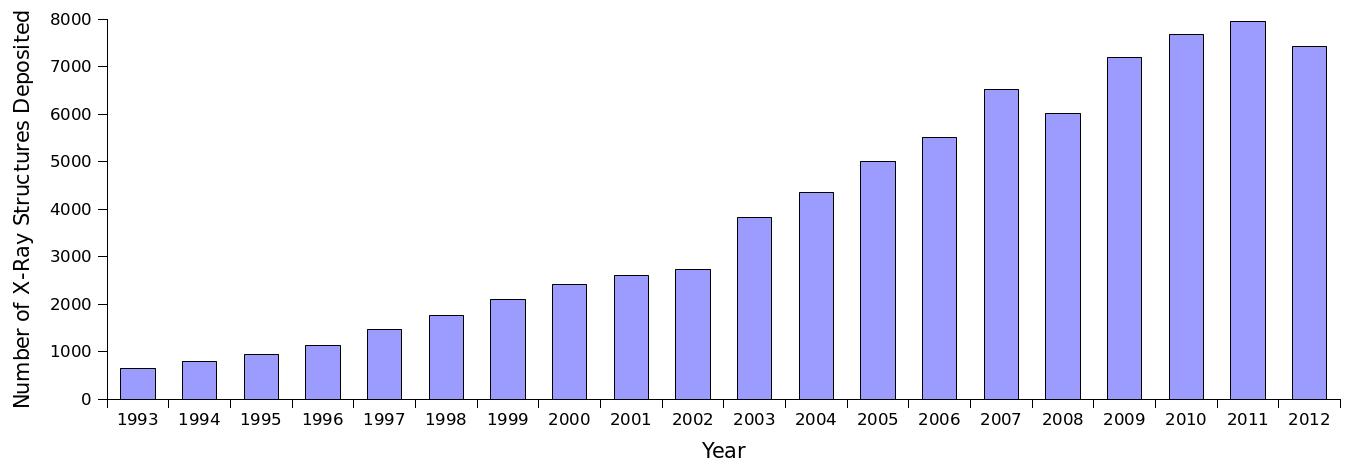
\includegraphics[width=\textwidth]{figures/pdb_deposit_rate.png}
\caption{The rate at which new structures is deposited into the PDB over the last two decades.
Due to a variety of improvements in the field of crystallography this rate has been steadily increasing.}
\label{figure:pdb_growth}
\end{center}
\end{figure}

For example a recent increase in the field of crystallography, is "crystal-less" crystallography in which small molecules are bound by a porous scaffold matrix.
The regular structure of the matrix imparts a regular packing arrangement, necessary for interpreting diffraction patterns, onto the arrangement of small molecules.
This has the potential to address one of the largest difficulties in obtaining quality structural data for proteins, which is that it is very difficult to purify and crystallize certain proteins \cite{inokuma2013x}.

The number of target molecules of the set of all drugs currently available on the market consists of only about 500 proteins.
The bottleneck in introduction of new chemical entities is not virtual screening, but rather optimizing these hits into higher affinity leads and eventually balancing the requirements across all characteristics to produce a new drug.
 \cite{bleicher2003hit}

Of the total proteome only ~30,000 are regulated by small molecule binding, making them reasonable targets of drug action.
A large number of these possible drug targets are not implicated in any disease, due to this and a number of other factors, estimates of the total number of these proteins which are possible drug targets is much lower.
Frequently cited numbers for the number of possible drug targets in humans are six-hundred to fifteen-hundred, still significantly higher than the total number of targets which are exploited by current drugs.
The different families of cellular proteins are not equally likely to be targets of drugs.
As of \the\year 47\% of current drug targets are enzymes, followed by 30\% being GPCR's \cite{hopkins2002druggable}.

The consists of a number of characteristics which are generally true of drug like molecules:
\begin{enumerate}
\item Five or fewer hydrogen bond donors,
\item 500 Da or less total molecular mass
\item high liphophilicity
\item sum of nitrogen and oxygen atoms is not greater than 10 \cite{rule_of_five}
\end{enumerate}

Through understanding the protein-ligand conformation and specific contacts they were able to modify a known substrate 
There is an advantage to flexible substrates, which is that they can flex in order to create better contacts with the protein structure increasing binding affinity.
This is especially important as the location of heavy atoms in the target protein is frequently only known to an accuracy of ~0.4 angstroms.
Further specific knowledge of the binding geometry between the initial lead compound and the target makes it possible to computationally screen possible chemical group substituents, to maximize binding affinity, increase solubility or bioavailability.
One of the earliest examples of the successful application of structure based drug design is the carbonic anhydrase inhibitor dorzolamide, in which most of these ideas were applied to find a drug with very high binding affinity \cite{greer1994application}.

Despite advantages in speed and cost due to limitations in accuracy computational screening has struggled to produce the same results as empirical screening.
However, more recently virtual screening has succeeded in producing hit rates greater than those from empirical screening techniques.
Virtual screening identified leads which were later developed into the human immunodeficiency virus (HIV) protease inhibitor Viracept, and the anti-influenza drug Relenza.
A number of challenges which limit the utility of docking programs have been identified
\begin{enumerate}
\item The number of possible small molecules is essentially unbounded, however only a very small fraction of these ligands are potentially drug compounds. Limiting sampling to this subspace is a challenging problem.
\item The number of conformations of ligand molecules rises exponentially with the number of internal degrees of freedom of the ligand. Sampling the huge conformational space of the ligand becomes a computationally difficult problem on its own.
\item The difficulty of accurately assessing or comparing the energy of different protein-ligand complexes or conformations.
\end{enumerate}
 \cite{shoichet2004virtual}
